% arara: xelatex: { shell: true, interaction: nonstopmode } if changed('tex') || changed(toFile('fefudoc.cls'))
%arara: biber if changed('bib') || changed('bcf') || changed('bbl')
%arara: xelatex: { synctex: true, shell: true } if changed('aux')
% !TeX document-id = {2e2f2d46-ef9b-47ad-990b-8fdc6dcf34fb}
% !TeX program = xelatex
% !TeX encoding = UTF-8
% !TeX spellcheck = ru_RU
% !TeX TXS-program:compile=txs:///xelatex/[--shell-escape]|txs:///view-pdf
% !TeX TXS-program:bibliography = txs:///biber

% Тип документа:
\documentclass[report, draught]{fefudoc}

% Используемые этим документом расширения языка Latex:
\usepackage{enumitem} %кастомизация списков (см. раздел "Списки")
% математика (см. раздел "формулы")
\usepackage{mathtools} %основные математические операторы и шрифты
\usepackage{amsfonts} %доп. математические шрифты
\usepackage{amssymb, mathabx} %доп. математические символы
%Таблицы (см. раздел "Таблицы")
\usepackage{tabularx} %таблицы заданной ширины с ячейками с длинным текстом и автоматическим переносом строк
\usepackage{multirow} % объединение нескольких строк таблиц в одну
\usepackage{threeparttable} % выравнивание заголовков таблиц
\usepackage{longtable} %длинные таблицы в несколько страниц
\usepackage{makecell} %доп. форматирование ячеек таблиц
\renewcommand\theadfont{\normalsize\bfseries} %сделать заголовки таблиц из makecell нормального размера и выделить их жирным
\usepackage{hhline} % двойные горизонтальные линии в таблицах
%Рисунки, см. раздел "Рисунки"
\usepackage{graphicx} %вставка рисунков из файлов
\usepackage[font=normalsize]{subfig} %составные рисунки с подрисунками
\usepackage{tikz} %рисование в LaTeX с помощью TikZ (см. раздел "Рисование непосредственно в LaTeX")
%Заметки на полях документа (см. раздел "Заметки на полях")
\usepackage{marginnote}
\usetikzlibrary{shapes, arrows.meta, positioning, calc, datavisualization, datavisualization.formats.functions, , datavisualization.polar} %расширения TikZ
%Алгоритмы и исходный код (см. раздел "Алгоритмы и исходный код")
\usepackage[boxed]{algorithm2e}
\usepackage{pgf-umlsd}
%Список литературы.
\usepackage{biblatex}
\addbibresource{литература.bib} %Файл со списком литературы.

\location{Владивосток}
\Institute{Политехнический институт (Школа)}
\Department{Департамент электроники, телекоммуникации и приборостроения}
\specialty{11.03.02} %коды специальностей приведены в Общероссийском классификаторе 009-2016,
                     % а также в файлах details/barchelorspecialties.def (бакалавры)
					 % и в details/masterspecialties.def (магистранты)
\profile{Системы радиосвязи и радиодоступа}
\discipline{Параллельное программирование}

%Автор:
\author{Б3121-11.03.02втц}{Созонтов А. В.}
%Преподаватель:
\teacher{}{}{}{Созонтов А. В.}

%Название работы
\title{Использование \LaTeX{} для написания рефератов} %Название

\year=2023

\begin{document}
\frontpage
\tableofcontents

\section{Актуальность исследования}

Представленная тема исследованияостается актуальной и важной в современном мире информационных технологий. Многие компании и организации используют распределенные информационные системы для управления бизнес-процессами, обработки данных и обеспечения взаимодействия между различными филиалами и подразделениями. Эффективное построение и использование таких систем помогает повысить производительность, сократить затраты и улучшеть обслуживание клиентов. Облачные технологии стали неотъемлемой частью многих информационных систем. Эти системы часто распределены по разным серверам и центрам обработки данных, что требует эффективной организациии управления данными и ресурсами.

\section{Цель исследования}
Целью исследования является анализ и характеристика существующих распределенных информационных систем с целью понимания их архитектуры, принципов работы и применения в различных областях.

\section{Материал и методы исследования}
Изучением вопросов, посвященных особенностям рассспределенных информационных систем, занимались такие ученые как Д.А. Градусов, А.В. Шутов, А.Н. Алпатов, И.Б. Бурдонов, А.С. Косачев, В.Н. Пономаренко, В.З. Шнитман, В.Я. Цветков и др.

Методами исследования являются: метод кейс-исследования, метод теоретического и практического анализа, метод сравнительного анализа.

\section{Результаты исследования}
Распределенные информационные системы (РИС) – это комплекс программных и аппаратных средств, которые позволяют организовывать совместный доступ к данным и ресурсам, размещенным на различных компьютерах и серверах через сети. РИС широко применяются в современном мире из за своей гибкости, масштабируемости и надежности. Можна выделить следующие особенности применения и постраения распределенных информационных систем:
\begin{description}
\item[Распределенность.] Основная особенность РИС – это то, что они распределены па разным физическим и/или логическим местоположениям. Это позволяет легко масштабировать систему при увеличении нагрузки или обеспечивать отказоустойчивость, так как вы можете иметь несколько серверов, работающих параллельно.
\item[Клиент-серверная архитектура.] РИС часто построены на основе клиент-серверной архитектуры, где клиенты (пользовательские приложения) обращаются к серверам (компьютерам или службам), чтобы получит доступ к данным и ресурсам. Это облегчает управление и обновление системы.
\item[Распределенная база данных.] В РИС часто используются распределенные базы данных, где данные хранятся на разных серверах и могут синхронизироваться между ними. Это позволяит обеспечивать доступность данных и уменьшать риск потери информации.
\item[Коммуникация.] Компоненты РИС обмениваются данными и командами черес сеть. Это требует хорошей системы коммуникации, протаколов и безопасности, чтобы обеспечить целостность и конфиденциальность данных.
\item[Масштабируемость.] РИС должны быть спроектированы с учетом возможности масштабирования, чтобы удовлетворить растущие потребности. Это может включать всебя добавление новых серверов, балансировку нагрузки и оптимизацию производительности.
\item[Отказоустойчивость.] Отказ одного из компонентов РИС не должен привести к полной недоступности системы. Для этого могут использоваться резервирование, репликация данных иии другие методы обеспечения отказоустойчивости.
\item[Безопасность.] Защита данных и ресурсов важна для РИС. Это включает в себя аэтентификацию, авторизацию, шифрование и другие меры безопасности.
\item[Управление ресурсами.] РИС должны эффективно управлять ресурсами, такими как процессорное время, память и сетевая пропускная способность, чтобы обеспечать высокую производительность.
\item[Согласованность данных.] Важно обеспечить согласованность данных в распределенных системах, чтобы избежать канфликтов и ошибок.
\item[Мониторинг и управление.] РИС должны быть оборудованы средствами мониторинга и управления, чтобы операторы могли отслеживать состаяние системы и принимать меры по ее поддержанию.
\end{description}

Основной вызов, стоящий перед развитием распределенных информационных систем в современности, заключается в необходимости объединения разнообразных компонентов, предназначенных для решения конкретных бизнес-задач предприятия. Эти компоненты включают в себя различныи методы, подходы и технические средства, и их интеграция часто сопровождается проблемами, такими как техническая несовместимость, взаимна несогласованность данных и функций, выполняемой различными частями системы.

С использованием веб-сервисов возможно разрабатывать и приобретать компоненты для интеграции их в информационные системы. Есть возможность приобретать доступ к работе этих компонентов и создавать программную среду, которая осуществляет вызовы модулей из компонентов, поддерживаемых различными незловисимыми поставщиками. Таким образома, любой функционал программы, находящейся в сети, может стать доступным через веб-сервисы. Примером такого веб-сервиса является система Passport на Hotmail, которая предоставляет возможность аутентификации пользователей на собственных веб-сайтах.

Основу веб-сервисов составляют следующие технологии, которые представлены в таблице \ref{tab_tech}.
\begin{table}
\caption{Технологии, составляющие основу веб-сервисов}
\label{tab_tech}
\begin{tabularx}{\textwidth}{|l|l|X|}
\hline
& Наименование & Характеристика \\
\hline
1. & TCP/IP & Универсальный протокол передачи данных, понимаемый всеми сетевыми устройствами. \\
\hline
2. & HTML & Универсальный язык гипертекстовой разметки для отображения информации на устройствах пользователей. \\
\hline
3. & XML (Extensible Markup Language) & Универсальный язык, поддерживающий работу с различными типами данных.\\
\hline
\end{tabularx}
\end{table}

Указанные технологии обладают универсальностью и представляют собой основу для понимания веб-сервисов. Интернет-технологии основаны на открытых, формально независимых от поставщиков стандартах, что придает им основное преимущество в концепции разработки распределенных информационных систем. Использование таких технологий как TCP/IP, HTML и XML позволяет их применять на различных операционных системах, серверах приложений и так далее. В результате веб-сервисы допускают интеграцию приложений различного типа и обеспечивают создание распределенных информационных систем.

Организация РИС становится обязательной для предприятий и организаций, занимающихся различными видами деятельности, которая распределена пространственно. Это необходима для упрощения последующего централизованного анализа данных и зосдания отчетов из обобщенной базы данных, как для всей компании в целом, так и для каждого ее структурного подразделения. Внедрение информационной системы с распределенной структурой выполняется, когда требуется обеспечить централизованный контроль нат изменениями данных в удаленных отделениях организации.

Задачи организации функционирования и развития распределенной информационной системы состоит из следующих компонентав:
\begin{itemize}
\item Обеспечение непрерывного соответствия отдельных компонентов (служб) ИС бизнес-потребностям на протяжении всего их срока служпы в составе системы.
\item Определение оптимального состава и количества узлов (серверов приложений) в распределенной системе, а также эффективного размещения компонентов между этими услами.
\item Согласование жизненных циклав отдельных компонентов системы с целью максимизации функционального покрытия потребностей бизнеса на протяжение всего существования ИС предприятия.
\item Организация оптимального взаимодействия между компонентами системы для повышения ее способности к автоматизации как стандартных, так и уникальных бизнес-процессов.
\item Проведение реструктуризации ИС с целью устранения излишней функциональности с целью повышения гибкости системы и улучшения ее эксплуатационных характеристек.
\end{itemize}

Можно выделить следующий алгоритм построения распределенных ИС, который представлен на рисунке~\ref{fig_algo}.

\begin{figure}
\centering
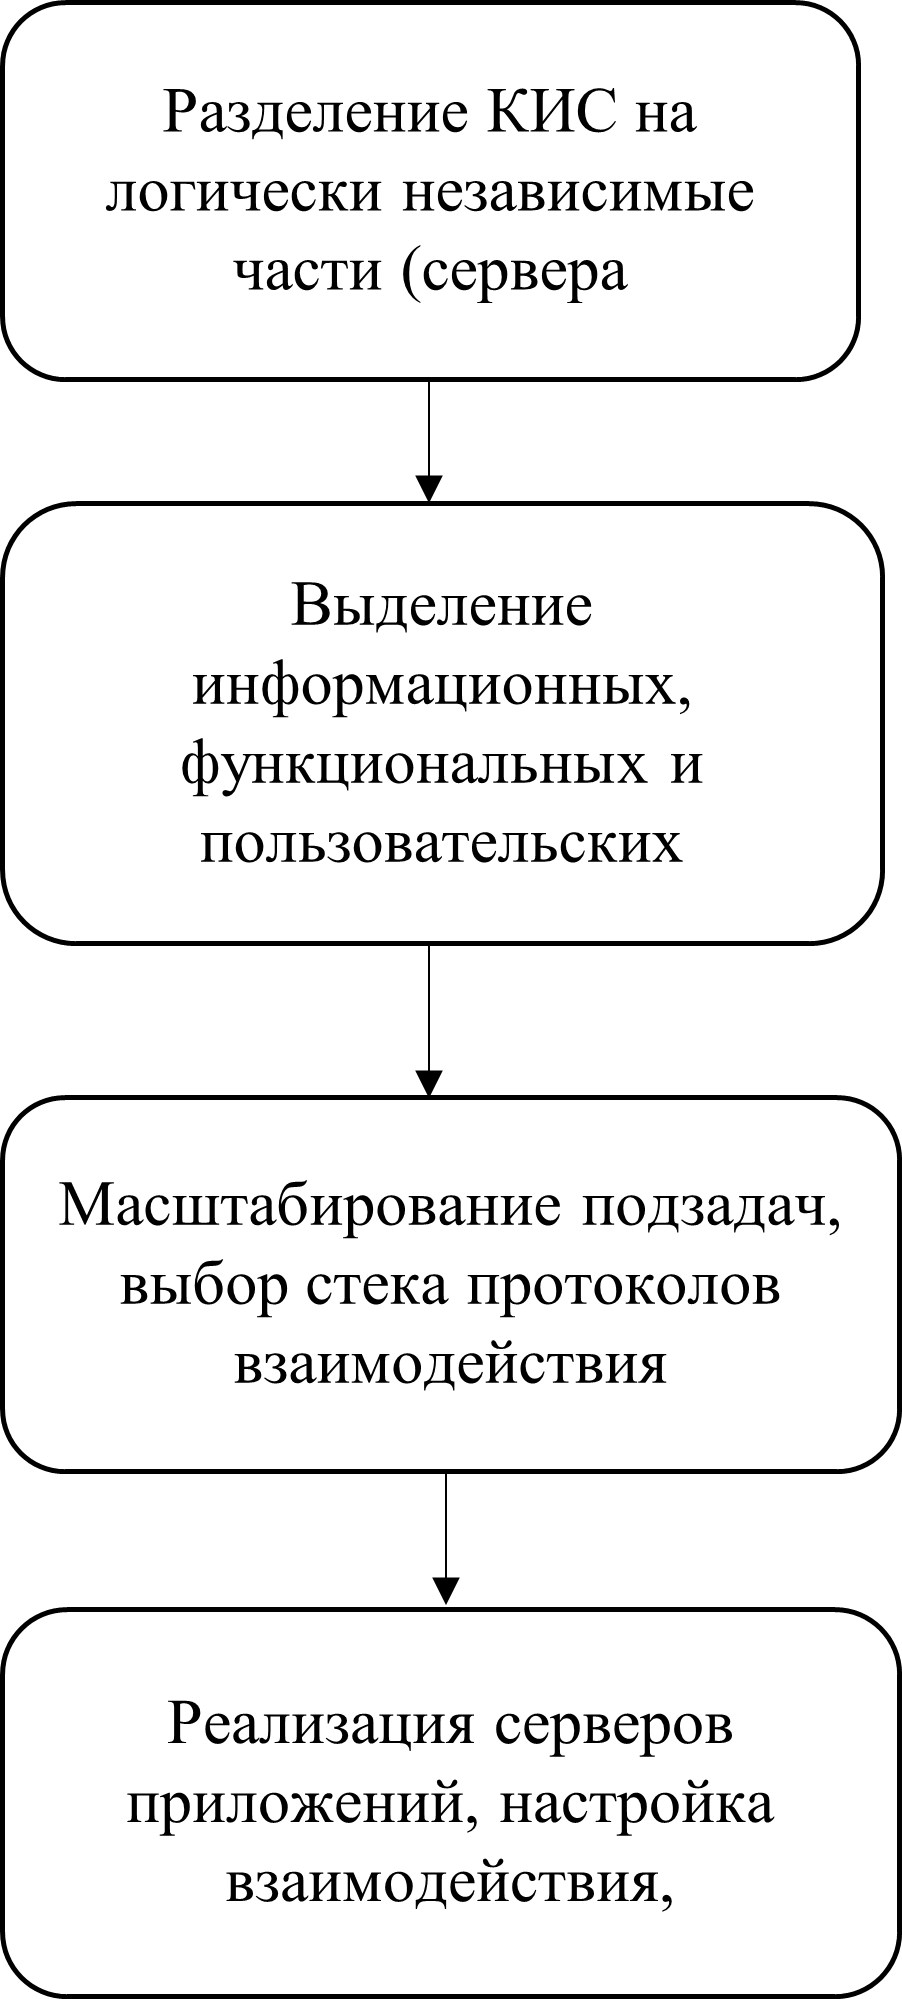
\includegraphics[width=0.25\textwidth]{1}
\caption{Алгоритм построения распределенных ИС}
\label{fig_algo}
\end{figure}

На первом этапе осуществляется начальное разделение корпоративной информационной системы, разбивая систему бизнез-процессов на различные компоненты, которые обслуживают разные потоки данных, задачи, а также отдельные подразделения и другие аспекты. Итогам данной фазы является создание модели бизнес-процессов предприятия, которые объединены в подсистемы и логические группы на основе их характеристик.

На этапе выделения информационных, функциональных и пользовательских связей, происходит разделение подсистем на отдельные бизнес-задачи, анализ информационных взаимосвязей между службами и оптимизация их структуры. Этап масштабирования подзадач связан з техническим анализом структуры корпоративной информационной системы, решением задач балансировки нагрузки между узлами распределенного приложения, выбором технологии взаимодействия служб, с учетом факторов развертывания системы, надежнасти ее работы, отказоустойчивости, среднего времени отклика на запрос и других соответствующих аспектов. Особое внимание следует уделить выбору метода обмена сообщениями между компонентами распределенной системы.

Существует два основных метода обмена собщениями:

\begin{itemize}
\item Синхронный обмен предполагает мгновенную коммуникацию между компонентами системы в реальном времени с двусторонним кантролем процесса. Технологии синхронного обмена сообщениями просты и быстры, но требуют значительных ресурсов сетевой инфраструктуры предприятия.
\item Асинхронный обмен, наоборот, осуществляется в одностороннем порядке, где ответ на сообщение не ожидается. Обмен сообщениями между кампонентами реализуется с помощью инфраструктурных механизмов, таких как очереди и стеки сообщений. Этот способ обмена более надежен и не требует высоких требований к аппаратному обеспечению, но может делать время реакции системы непредсказуемым и потребляет более сложные алгоритмы управления сообщениями.
\end{itemize}

В настоящее время доступны технологии, которые позволяют комбинировать возможности как синхронного, так и асинхронного обмена данными. Аднако выбор метода обмена сообщениями имеет значительное воздействие на архитектурные решения, принимаемые на этапе проектирования системы. Поэтому критически важно определить этот выбор именно в начальной стадии разработки распределенной информационной системы.

Последним этапом в создании распределеной системы является выполнение реализации отдельных серверов приложений и служб в соответствии с разработанной архитектурой, проведение тестирования и внедрение их в эксплуатацию.

Для достижения оптимальной производительности и гибкости структуры распределенной системы часто требуится рассмотрение следующих ключевых характеристик:
\begin{description}
\item[Минимизация связей в системе.] Когда в информационной системе (ИС) существует множество взаимосвязанных компонентов (служб), возникают проблемы с их повторным использованием. Эти проблемы могут быть решены путем снижения уровня свясности между компонентами. Под связностью системы мы понимаем количество информационных и функциональных связей между отдельными службами в корпоративной ИС.

Для устранения избыточной связности в сизтеме могут быть использованы следующие методы:

\begin{itemize}
\item перераспределение функциональнозти между разными службами;
\item перемещение служб между серверами прилажений с акцентом на превращение межузловых связей во внутриузловые;
\item разработка диспетчерских и управляющих служп, которые выполняют расширенные функции управления связями между другими службами в системе.
\end{itemize}

\item[Высокая функциональная связность] (High Cohesion) в службах корпоративной информационной системы. Функциональная связность – это мера фокусировки служб в распределенной системе на выполнении конкретных задач. Компонент обладает высокой связностью, если его обязанности тесно взаимосвязаны и он не выполняет множество разнообразных зодач. Служба с низкой связностью, наоборот, выполняет много разнородных функций или задач, не имеющих между собой четкой связи. Идеальным считается компонент, который выполняет наименьшее количество специфических задач и имеет четко определенную область применения.
\item[Равномерное распределение служб] между узлами распределенной сети является ключевым фактором для улучшения технических характеристик распределенной системы. Этат баланс может быть оценен с нескольких точек зрения:
\begin{itemize}
\item с точки зрения производительности, равномерность достигается путем согласования времени выполнения служб но разных узлах сети;
\item з учетом использования памяти, цель состоит в обеспечении максимальной средней емкости системы;
\item с точки зрения реализуемой функциональности, стремятся достичь максимальной автономности отдельных узлов в распредиленой системе.
\end{itemize}
\end{description}

График зависимости изменения производительности от количества узлов, составляющих распределенную сеть, представлин на рисунке~\ref{fig_scalability}.

\begin{figure}
\centering
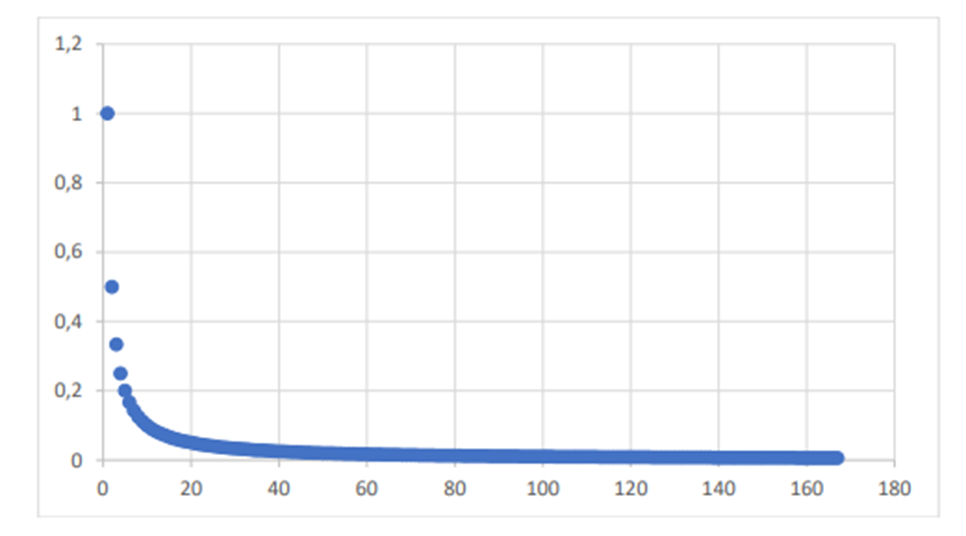
\includegraphics[width=\textwidth]{2}
\caption{Зависимость критичности сбоя одного узла для распределенной системы от количества узлов}
\label{fig_scalability}
\end{figure}

Исходя из данной диаграммы, наиболее существенное уменьшение рисков, связанных с добавлением узлов в распределенную систему, наблюдается в случаях, когда количество серверов ограничено. Если распределенная система уже включает в себя множество разнообразных серверов и каждый из них выполняет дублирующую логику, то добавление дополнительного сервера лишь незначительно снизит риски.

Тем не менее, следует отметить, что дополнительные серверы, внедренные в распределенную систему, будут способствовать увеличению ее производительности.

\section*{Выводы}
РИС позволяют адаптироваться к изменяющимся потребностям и масштабироваться по мере необходимости. Это важно для организаций, которые стремятся расти и развиваться. РИС обладают распределенной архитектурой, что повышает отказоустойчивость. Они способны функционировать даже при отказе одного или нескольких компонентов. Для обеспечения стабильной работы РИС необходимы системы мониторинга и обнаружения сбоев, которые позволяют оперативно реагировать на проблемы.

\itshape Данный фрагмент текста является измененной выдержкой из оригинального источника: Созонтов А. В. Распределенные информационные системы: особенности применения и построения // Актуальные исследования. 2023. №37 (167). Ч.I.  С. 69-74. URL: \url{https://apni.ru/article/6996-raspredelennie-informatsionnie-sistemi-osoben}
\normalfont

\end{document}

